% =====================================================================
%  Chapter 1: Points, Vectors, and Space
% =====================================================================

\chapter{Points, Vectors, and Space}
\label{ch:1}

\section{Why multivariable calculus begins with geometry}

Single-variable calculus lived on a line.  A point was described by one number, and
there were only two directions to move: left or right. But many real-life questions do not
live on a real line.  A storm moves across a map, a satellite moves through space, and
the temperature in a room depends on where you stand.

\subsection{From one input to many inputs}

Imagine a small weather station on the coast.  A radar image says that the center of
a storm cell is
\[
    12 \text{ km east}, \qquad 5 \text{ km north}
\]
of the station. The location is naturally written as the
ordered pair
\[
    P=(12,5).
\]
A helicopter hovering above the same point needs a third number.  If it is
\(0.8\) km above the ground, its position is
\[
    H=(12,5,0.8).
\]

The numbers in these lists do not all have the same meaning.  The first two numbers
locate a point on a flat map.  The third number locates height.  But the idea is the
same: a position is described by several coordinates.

\begin{figure}[h]
\centering
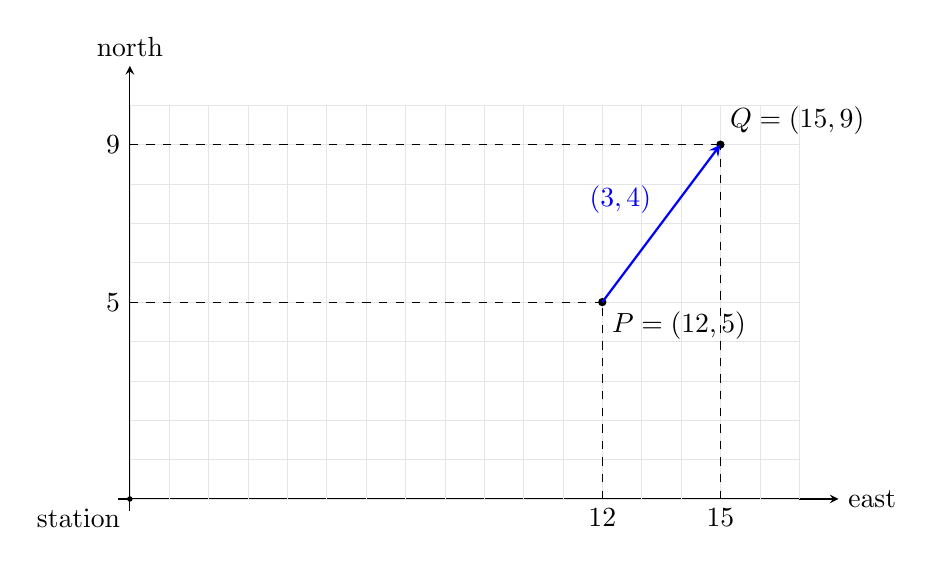
\begin{tikzpicture}[scale=0.5, >=stealth] % Reduced scale slightly to fit the page width
    % Expanded axes to accommodate Q=(15,9)
    \draw[->] (-0.3,0) -- (18,0) node[right] {east};
    \draw[->] (0,-0.3) -- (0,11) node[above] {north};

    % Expanded grid
    \draw[step=1, gray!20, very thin] (0,0) grid (17,10);

    % Point P
    \fill (12,5) circle (3pt);
    \node[below right] at (12,5) {\(P=(12,5)\)};
    \draw[dashed] (12,0) -- (12,5);
    \draw[dashed] (0,5) -- (12,5);
    \node[below] at (12,0) {\(12\)};
    \node[left] at (0,5) {\(5\)};

    % Point Q
    \fill (15,9) circle (3pt);
    \node[above right] at (15,9) {\(Q=(15,9)\)};
    \draw[dashed] (15,0) -- (15,9);
    \draw[dashed] (0,9) -- (15,9);
    \node[below] at (15,0) {\(15\)};
    \node[left] at (0,9) {\(9\)};

    % Displacement Vector (Optional, but helpful for Section 10.1.2)
    \draw[->, thick, blue] (12,5) -- (15,9) node[midway, above left] {\((3,4)\)};

    \fill (0,0) circle (2pt);
    \node[below left] at (0,0) {station};
\end{tikzpicture}
\caption{The storm moves from $P$ to $Q$, requiring a larger coordinate grid.}
\end{figure}

This is the first reason multivariable calculus begins with geometry.  Before we can
differentiate or integrate, we need to know where things are.

\subsection{Position, displacement, and measured quantities}

Now suppose the storm moves.  One hour later its center is
\[
    Q=(15,9).
\]
We can subtract the coordinates to find the displacement:
\[
    Q-P=(15-12,\;9-5)=(3,4).
\]
That means the storm moved \(3\) km east and \(4\) km north.

If it moved in a straight line, the distance traveled is found from the same
Pythagorean theorem used in the plane:
\[
    \sqrt{3^2+4^2}=5 \text{ km}.
\]

\begin{example}[A storm displacement]
The point
\[
    P=(12,5)
\]
is a location.  The ordered pair
\[
    (3,4)
\]
is a displacement.  It tells us how to move from \(P\) to \(Q\):
\[
    (12,5)+(3,4)=(15,9).
\]
The same displacement could start somewhere else:
\[
    (2,1)+(3,4)=(5,5).
\]
So a displacement is not tied to one fixed place.  It can be applied to any point.
\end{example}

This distinction is small, but it will save us from confusion later.

A \emph{point} is a location.  A \emph{vector} is a displacement.  Coordinates let us
write both with ordered lists, but the meanings are different.

\subsection{A first story: locating a storm, a satellite, and a temperature reading}

The same coordinates can also be used as inputs to a function.

At the point \((12,5)\), a weather sensor might report a temperature of
\(18^\circ\)C.  Then temperature is not itself a point.  It is a number assigned to a
point:
\[
    T(12,5)=18.
\]
If the temperature is measured over a whole region, we have a function
\[
    T(x,y).
\]
The input is a point on a map, and the output is a number.

A satellite position is different.  At time \(t\), the satellite has three coordinates:
\[
    \mathbf r(t)=(x(t),y(t),z(t)).
\]
Here the input is one number, time, but the output is a point in space.

So several kinds of functions will appear in this book:
\[
\begin{array}{c|c|c}
\text{Situation} & \text{Input} & \text{Output} \\ \hline
\text{temperature on a map} & (x,y) & T(x,y) \\
\text{height of a hill} & (x,y) & z=f(x,y) \\
\text{satellite motion} & t & \mathbf r(t)=(x(t),y(t),z(t)) \\
\text{wind in the plane} & (x,y) & \mathbf F(x,y)
\end{array}
\]

The last example is especially important.  A wind field assigns an arrow to every
point.  At one point the wind may blow east; at another, northeast; at another, not
at all.  Later, this idea will become a \emph{vector field}.  Vector fields are the
natural language of fluids, force, electricity, magnetism, and many of the integral
theorems near the end of the book.

\subsection{What changes from single-variable calculus, and what stays the same}

Single-variable calculus asked questions like these:
\[
    \text{How fast is } f(x) \text{ changing?}
\]
and
\[
    \text{How much has accumulated from } a \text{ to } b?
\]

Those questions remain.  But the geometry changes.

For a function of one variable, the graph is a curve in the plane.  At a point, there
is one main direction to move along the input line.  For a function of two variables,
the graph is usually a surface in space.  At a point in the input plane, there are
infinitely many directions to move.

A hiker standing on a hillside can walk north, south, east, west, or along any slanted
path between them.  A single slope number no longer tells the whole story.

The old ideas will return in new forms:
\[
\begin{array}{c|c}
\text{Single-variable calculus} & \text{Multivariable calculus} \\ \hline
\text{number line} & \text{plane and space} \\
\text{slope of a curve} & \text{rates of change in many directions} \\
\text{tangent line} & \text{tangent planes and tangent spaces} \\
\text{area under a graph} & \text{area, volume, flux, and circulation} \\
\int_a^b f'(x)\,dx=f(b)-f(a) &
\text{boundary integrals equal interior integrals}
\end{array}
\]

The last line is the long story of the book.  The Fundamental Theorem of Calculus
will not disappear.  It will grow.

For now, the next step is much simpler.  The difference between two locations behaves
like a reusable instruction:
\[
    \text{move } 3 \text{ east and } 4 \text{ north}.
\]
That instruction is the first object we need to understand carefully.  It is called a
\emph{vector}.

\section{Vectors in the plane and in space}

The storm story in the previous section used two kinds of objects.  Points told us
where something was.  Displacements told us how to move from one point to another.
Those displacements are the vectors.

\subsection{Vectors as arrows, displacements, and ordered lists}

A drone starts at
\[
    P=(1,2,1)
\]
where the coordinates are measured in meters: east, north, and up.  It receives the
instruction
\[
    \mathbf v=(4,-1,3).
\]
This means:
\[
    4 \text{ meters east}, \qquad 1 \text{ meter south}, \qquad 3 \text{ meters up}.
\]
After carrying out the instruction, the drone is at
\[
    P+\mathbf v=(1,2,1)+(4,-1,3)=(5,1,4).
\]

\begin{example}[The same vector in different places]
The vector
\[
    \mathbf v=(4,-1,3)
\]
can be drawn with its tail at the point \((1,2,1)\), but it does not belong only
there.  If the same drone instruction starts at
\[
    A=(10,0,2),
\]
then the endpoint is
\[
    A+\mathbf v=(14,-1,5).
\]
The arrow has moved, but the displacement is the same.
\end{example}

\begin{definition}[Vectors in \(\mathbb R^2\) and \(\mathbb R^3\)]
A vector in the plane is an ordered pair
\[
    \mathbf v=(v_1,v_2).
\]
A vector in space is an ordered triple
\[
    \mathbf v=(v_1,v_2,v_3).
\]
The numbers \(v_1,v_2,v_3\) are called the \emph{components} of the vector.
\end{definition}

The zero vector is
\[
    \mathbf 0=(0,0)
\]
in the plane and
\[
    \mathbf 0=(0,0,0)
\]
in space.  It means no displacement.

\subsection{Addition and scalar multiplication}

Suppose a kayak moves through still water with displacement
\[
    \mathbf p=(3,1)
\]
during a short time interval.  At the same time, the current pushes it by
\[
    \mathbf c=(1,2).
\]
The actual displacement is
\[
    \mathbf p+\mathbf c=(3,1)+(1,2)=(4,3).
\]
Vector addition adds the motions component by component.

\begin{definition}[Vector addition and scalar multiplication]
For vectors in the plane,
\[
    \mathbf u=(u_1,u_2), \qquad \mathbf v=(v_1,v_2),
\]
their sum is
\[
    \mathbf u+\mathbf v=(u_1+v_1,\;u_2+v_2).
\]
If \(c\) is a number, then
\[
    c\mathbf u=(cu_1,\;cu_2).
\]
The same rules hold in space:
\[
    (u_1,u_2,u_3)+(v_1,v_2,v_3)
    =(u_1+v_1,\;u_2+v_2,\;u_3+v_3),
\]
and
\[
    c(u_1,u_2,u_3)=(cu_1,\;cu_2,\;cu_3).
\]
\end{definition}

Geometrically, \(\mathbf u+\mathbf v\) is found by placing the tail of \(\mathbf v\)
at the head of \(\mathbf u\).  The combined displacement goes from the first tail to
the last head.

\begin{figure}[h]
\centering
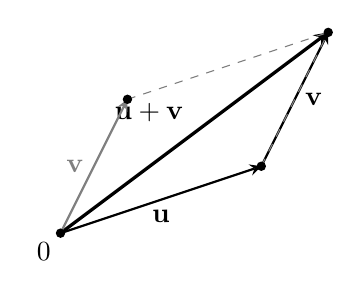
\begin{tikzpicture}[scale=0.85, >=stealth]
    \coordinate (O) at (0,0);
    \coordinate (U) at (3,1);
    \coordinate (V) at (1,2);
    \coordinate (UV) at (4,3);

    \draw[->, thick] (O) -- (U) node[midway, below] {\(\mathbf u\)};
    \draw[->, thick] (U) -- (UV) node[midway, right] {\(\mathbf v\)};
    \draw[->, very thick] (O) -- (UV) node[midway, above left] {\(\mathbf u+\mathbf v\)};

    \draw[->, thick, gray] (O) -- (V) node[midway, left] {\(\mathbf v\)};
    \draw[dashed, gray] (V) -- (UV);
    \draw[dashed, gray] (U) -- (UV);

    \fill (O) circle (2pt);
    \fill (U) circle (2pt);
    \fill (V) circle (2pt);
    \fill (UV) circle (2pt);

    \node[below left] at (O) {\(0\)};
\end{tikzpicture}
\caption{Adding vectors by placing arrows head-to-tail.}
\end{figure}

Multiplying by \(c\) stretches or reverses a vector.  For example, if
\[
    \mathbf u=(3,1),
\]
then
\[
    2\mathbf u=(6,2), \qquad -\mathbf u=(-3,-1), \qquad \frac12\mathbf u=\left(\frac32,\frac12\right).
\]
The vector \(2\mathbf u\) points in the same direction as \(\mathbf u\) and is twice
as long.  The vector \(-\mathbf u\) points in the opposite direction.

\subsection{Linear combinations and spans}

A city map gives two basic walking instructions:
\[
    \mathbf e=(1,0), \qquad \mathbf n=(0,1).
\]
Here \(\mathbf e\) means one block east, and \(\mathbf n\) means one block north.
Then
\[
    4\mathbf e+3\mathbf n=(4,0)+(0,3)=(4,3).
\]
So the instruction ``walk 4 blocks east and 3 blocks north'' is built from the two
basic directions.

\begin{definition}[Linear combination]
A vector of the form
\[
    a\mathbf u+b\mathbf v
\]
is called a \emph{linear combination} of \(\mathbf u\) and \(\mathbf v\).  The numbers
\(a\) and \(b\) are called \emph{coefficients}.
\end{definition}

The same idea works with more vectors:
\[
    a\mathbf u+b\mathbf v+c\mathbf w.
\]
A linear combination is just a recipe: take some amount of each vector and add the
results.

\begin{example}[Two directions may fill the plane]
Every vector \((x,y)\) in the plane can be written as
\[
    (x,y)=x(1,0)+y(0,1).
\]
So the two basic vectors
\[
    (1,0), \qquad (0,1)
\]
can build every displacement in the plane.
\end{example}

\begin{definition}[Span]
The \emph{span} of vectors \(\mathbf u\) and \(\mathbf v\) is the set of all their
linear combinations:
\[
    \operatorname{span}\{\mathbf u,\mathbf v\}
    =
    \{a\mathbf u+b\mathbf v : a,b\in\mathbb R\}.
\]
For one vector,
\[
    \operatorname{span}\{\mathbf u\}
    =
    \{a\mathbf u : a\in\mathbb R\}.
\]
\end{definition}

The word \emph{span} means ``all the places these directions can reach if we are
allowed to scale them and add them.''

\subsection{Lines through the origin and planes through the origin}

Start with one nonzero vector in the plane:
\[
    \mathbf u=(2,1).
\]
Its span is
\[
    \operatorname{span}\{\mathbf u\}
    =
    \{t(2,1):t\in\mathbb R\}.
\]
Writing out a few values gives
\[
\begin{array}{c|c}
t & t(2,1) \\ \hline
-1 & (-2,-1)\\
0 & (0,0)\\
1 & (2,1)\\
2 & (4,2)
\end{array}
\]
All of these points lie on one line through the origin.

\[
    \operatorname{span}\{(2,1)\}
\]
is the line through the origin in the direction \((2,1)\).

\begin{figure}[h]
\centering
\begin{tikzpicture}[scale=0.75, >=stealth]
    \draw[->] (-4,0) -- (5,0) node[right] {\(x\)};
    \draw[->] (0,-2.5) -- (0,3) node[above] {\(y\)};

    \draw[thick] (-4,-2) -- (5,2.5);
    \draw[->, very thick] (0,0) -- (2,1) node[right, below] at (2.6,1.1) {\(\mathbf u=(2,1)\)};

    \fill (0,0) circle (2pt);
    \fill (2,1) circle (2pt);
    \fill (4,2) circle (2pt);
    \fill (-2,-1) circle (2pt);

    \node[below right] at (-0.2,0.1) {\(0\)};
    \node[above right] at (3.5,2.1) {\(2\mathbf u\)};
    \node[below left] at (-1.9,-1.0) {\(-\mathbf u\)};
\end{tikzpicture}
\caption{The span of one nonzero vector is a line through the origin.}
\end{figure}

In space, one nonzero vector also spans a line through the origin.  Two genuinely
different directions can span a plane.  For example,
\[
    \mathbf u=(1,0,0), \qquad \mathbf v=(0,1,0).
\]
Then
\[
    a\mathbf u+b\mathbf v
    =
    a(1,0,0)+b(0,1,0)
    =
    (a,b,0).
\]
This is the \(xy\)-plane:
\[
    z=0.
\]

\begin{definition}[Lines and planes through the origin]
If \(\mathbf u\neq \mathbf 0\), then
\[
    \{t\mathbf u:t\in\mathbb R\}
\]
is the line through the origin in the direction \(\mathbf u\).

If \(\mathbf u\) and \(\mathbf v\) are not multiples of each other, then
\[
    \{s\mathbf u+t\mathbf v:s,t\in\mathbb R\}
\]
is the plane through the origin spanned by \(\mathbf u\) and \(\mathbf v\).
\end{definition}

The condition ``not multiples of each other'' matters.  If
\[
    \mathbf u=(1,2,0), \qquad \mathbf v=(2,4,0),
\]
then
\[
    \mathbf v=2\mathbf u.
\]
The two vectors look like two directions, but they are really the same direction with
different lengths.  Their span is still only a line, not a plane.

This is our first encounter with redundancy.  Later we will give it a name:
\emph{linear dependence}.

\subsection{Affine lines and affine planes: translating a span}

So far, every line and plane passed through the origin.  Most lines and planes do not.

A trail in space starts at the campsite
\[
    P=(1,2,0)
\]
and follows the direction
\[
    \mathbf u=(2,0,1).
\]
A point on the trail has the form
\[
    P+t\mathbf u
    =
    (1,2,0)+t(2,0,1).
\]
For example,
\[
    t=0 \quad \Rightarrow \quad (1,2,0),
\]
and
\[
    t=3 \quad \Rightarrow \quad (1,2,0)+3(2,0,1)=(7,2,3).
\]

The expression
\[
    P+t\mathbf u
\]
means: start at the point \(P\), then move by the vector \(t\mathbf u\).

\begin{definition}[Affine lines and affine planes]
Let \(P\) be a point.

The affine line through \(P\) in the direction \(\mathbf u\neq \mathbf 0\) is
\[
    P+\operatorname{span}\{\mathbf u\}
    =
    \{P+t\mathbf u:t\in\mathbb R\}.
\]

If \(\mathbf u\) and \(\mathbf v\) are not multiples of each other, the affine plane
through \(P\) in the directions \(\mathbf u\) and \(\mathbf v\) is
\[
    P+\operatorname{span}\{\mathbf u,\mathbf v\}
    =
    \{P+s\mathbf u+t\mathbf v:s,t\in\mathbb R\}.
\]
\end{definition}

The word \emph{affine} means that we have translated a line or plane away from the
origin.  The direction is still controlled by vectors.  The starting location is controlled
by the point \(P\).

\begin{example}[A translated plane]
Let
\[
    P=(0,0,2), \qquad \mathbf u=(1,0,0), \qquad \mathbf v=(0,1,0).
\]
Then
\[
    P+s\mathbf u+t\mathbf v
    =
    (0,0,2)+s(1,0,0)+t(0,1,0)
    =
    (s,t,2).
\]
This is the horizontal plane
\[
    z=2.
\]
It has the same directions as the \(xy\)-plane, but it has been lifted two units upward.
\end{example}

Vectors let us talk about direction without caring where the arrow is drawn.  Points
let us anchor those directions to actual places.  This is enough to describe many lines
and planes, but something is still hidden: the coordinates themselves.  Writing
\((3,2)\) quietly assumes that we have chosen an east direction, a north direction, and
a unit of measurement.  Change those choices, and the same geometric vector may get
different coordinates.  The next task is to understand what coordinates are really doing.
\section{Coordinates and dimension}

The last section ended with a quiet warning.  A vector can be drawn as an arrow, but
its coordinates depend on the directions and units we choose.  Coordinates are not the
vector itself; they are the vector written in a particular language.

That language is still powerful.  It lets us describe locations, directions, lines, planes,
and higher-dimensional data with the same simple algebra.

\subsection{The spaces \(\mathbb R^2\), \(\mathbb R^3\), and \(\mathbb R^n\)}

A small warehouse robot moves along three natural directions: east-west, north-south,
and up-down.  If it starts at the charging station and moves to
\[
    (7,3,2),
\]
we may read this as
\[
    7 \text{ meters east}, \qquad 3 \text{ meters north}, \qquad 2 \text{ meters up}.
\]
The same list of numbers could describe a point, if we are locating the robot, or a
vector, if we are describing a displacement.

Two coordinates give the plane:
\[
    \mathbb R^2=\{(x,y):x,y\in\mathbb R\}.
\]
Three coordinates give ordinary space:
\[
    \mathbb R^3=\{(x,y,z):x,y,z\in\mathbb R\}.
\]
There is no reason to stop at three coordinates.  A weather station might record
\[
    (\text{temperature},\text{pressure},\text{humidity},\text{wind speed}),
\]
which is a point in a four-dimensional data space.  We cannot draw four perpendicular
axes on a page, but the algebra still works.

\begin{definition}[The coordinate space \(\mathbb R^n\)]
For a positive integer \(n\), the space \(\mathbb R^n\) is the set of all ordered lists
of \(n\) real numbers:
\[
    \mathbb R^n
    =
    \{(x_1,x_2,\ldots,x_n):x_1,x_2,\ldots,x_n\in\mathbb R\}.
\]
The numbers \(x_1,x_2,\ldots,x_n\) are called the \emph{coordinates} of the point,
or the \emph{components} of the vector.
\end{definition}

The notation is the same for points and vectors because the same ordered lists are used
for both.  The meaning comes from the sentence around the notation.

For example,
\[
    P=(7,3,2)
\]
may mean a location in the warehouse.  But
\[
    \mathbf v=(7,3,2)
\]
may mean a displacement: move \(7\) east, \(3\) north, and \(2\) up.

This is why we often use letters like \(P,Q,A,B\) for points and bold letters like
\(\mathbf u,\mathbf v,\mathbf w\) for vectors.  The notation helps us remember the
difference, even though the coordinates look alike.

\subsection{Standard basis vectors}

On a map, the coordinate pair \((3,2)\) can be built from two basic moves:
\[
    3(1,0)+2(0,1)=(3,0)+(0,2)=(3,2).
\]
The vector \((1,0)\) means one unit in the first coordinate direction.  The vector
\((0,1)\) means one unit in the second coordinate direction.

These two vectors are so common that they get special names:
\[
    \mathbf e_1=(1,0), \qquad \mathbf e_2=(0,1).
\]
In space we use
\[
    \mathbf e_1=(1,0,0), \qquad
    \mathbf e_2=(0,1,0), \qquad
    \mathbf e_3=(0,0,1).
\]

\begin{figure}[h]
\centering
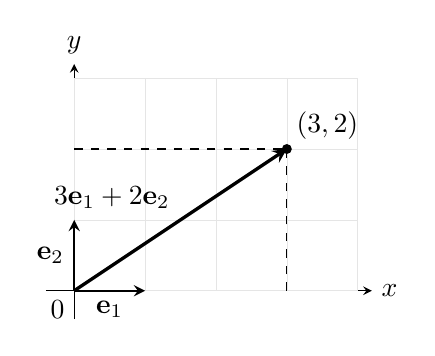
\begin{tikzpicture}[scale=0.9, >=stealth]
    \draw[->] (-0.4,0) -- (4.2,0) node[right] {\(x\)};
    \draw[->] (0,-0.4) -- (0,3.2) node[above] {\(y\)};

    \draw[step=1, gray!20, very thin] (0,0) grid (4,3);

    \draw[->, thick] (0,0) -- (1,0) node[midway, below] {\(\mathbf e_1\)};
    \draw[->, thick] (0,0) -- (0,1) node[midway, left] {\(\mathbf e_2\)};

    \draw[->, very thick] (0,0) -- (3,2) node[midway, above left] {\(3\mathbf e_1+2\mathbf e_2\)};
    \draw[dashed] (3,0) -- (3,2);
    \draw[dashed] (0,2) -- (3,2);

    \fill (3,2) circle (2pt);
    \node[above right] at (3,2) {\((3,2)\)};
    \node[below left] at (0,0) {\(0\)};
\end{tikzpicture}
\caption{The standard basis vectors build the usual coordinates in the plane.}
\end{figure}

\begin{definition}[Standard basis vectors]
In \(\mathbb R^n\), the standard basis vector \(\mathbf e_j\) is the vector whose
\(j\)-th component is \(1\) and whose other components are \(0\):
\[
    \mathbf e_j=(0,\ldots,0,1,0,\ldots,0).
\]
\end{definition}

Every vector in \(\mathbb R^n\) is built from the standard basis vectors:
\[
    (x_1,x_2,\ldots,x_n)
    =
    x_1\mathbf e_1+x_2\mathbf e_2+\cdots+x_n\mathbf e_n.
\]
This formula is more than notation.  It says that coordinates are instructions:
\[
    x_1 \text{ steps in direction } \mathbf e_1,\quad
    x_2 \text{ steps in direction } \mathbf e_2,\quad
    \ldots
\]
The standard coordinate system is the grid made from these standard directions.

\begin{example}[A displacement in space]
A drone displacement is
\[
    \mathbf v=(4,-1,3).
\]
Using the standard basis in \(\mathbb R^3\),
\[
    \mathbf v
    =
    4\mathbf e_1-\mathbf e_2+3\mathbf e_3.
\]
So the command says: move \(4\) units in the first direction, \(-1\) unit in the
second direction, and \(3\) units in the third direction.
\end{example}

\subsection{Coordinate descriptions of geometric objects}

Coordinates let us describe entire geometric objects, not only single points.

A walking path in the plane starts at
\[
    P=(2,1)
\]
and follows the direction
\[
    \mathbf u=(3,2).
\]
The affine line from the previous section is
\[
    P+t\mathbf u=(2,1)+t(3,2).
\]
Writing out the coordinates gives
\[
    x=2+3t,\qquad y=1+2t.
\]
This is a \emph{parametric} description of the line.  The parameter \(t\) is a clock for
the motion along the line.

We can also remove \(t\).  From
\[
    x=2+3t
\]
we get
\[
    t=\frac{x-2}{3}.
\]
Substituting into \(y=1+2t\),
\[
    y=1+\frac{2(x-2)}{3}.
\]
After simplifying,
\[
    2x-3y=1.
\]
So the same line has two descriptions:
\[
    \boxed{(x,y)=(2,1)+t(3,2)}
\]
and
\[
    \boxed{2x-3y=1.}
\]

The parametric description tells us how to move along the line.  The equation tells us
how to test whether a point lies on the line.

\begin{example}[A plane from two directions]
A tilted sheet of metal passes through the point
\[
    P=(1,0,2)
\]
and contains the two directions
\[
    \mathbf u=(1,2,0), \qquad \mathbf v=(0,1,1).
\]
Points on the sheet have the form
\[
    P+s\mathbf u+t\mathbf v.
\]
Writing out the coordinates,
\[
    (x,y,z)
    =
    (1,0,2)+s(1,2,0)+t(0,1,1),
\]
so
\[
    x=1+s,\qquad y=2s+t,\qquad z=2+t.
\]
From the first and third equations,
\[
    s=x-1,\qquad t=z-2.
\]
Substitute these into the equation for \(y\):
\[
    y=2(x-1)+(z-2)=2x+z-4.
\]
Thus the same plane can be written as
\[
    \boxed{(x,y,z)=(1,0,2)+s(1,2,0)+t(0,1,1)}
\]
or as
\[
    \boxed{2x-y+z=4.}
\]
\end{example}

Equations and inequalities describe regions too.  For example,
\[
    0\leq x\leq 12,\qquad
    0\leq y\leq 8,\qquad
    0\leq z\leq 3
\]
describes a rectangular room that is \(12\) units long, \(8\) units wide, and \(3\) units
high.

The set
\[
    z=2
\]
is a horizontal plane.  The set
\[
    x=5
\]
is a vertical plane.  The set
\[
    x^2+y^2=1
\]
in \(\mathbb R^3\) is a cylinder of radius \(1\) around the \(z\)-axis.  The equation
does not mention \(z\), so \(z\) is free to take any value.

This is a useful habit: when an equation does not mention one coordinate, the object
extends freely in that coordinate direction.

\subsection{When a picture stops being possible: why \(\mathbb R^n\) still works}

The plane is easy to draw.  Space is harder, but still visible.  Four-dimensional space
is different.  There is no honest picture of four perpendicular coordinate axes in our
ordinary three-dimensional world.

But many useful objects are naturally four-dimensional or higher.

A sensor in a greenhouse might record
\[
    (T,p,h,c),
\]
where
\[
    T=\text{temperature},\quad
    p=\text{pressure},\quad
    h=\text{humidity},\quad
    c=\text{carbon dioxide level}.
\]
This point lives in \(\mathbb R^4\).  A small change in the sensor reading might be
\[
    \Delta \mathbf s=(2,-0.1,5,0.03).
\]
That means temperature rose by \(2\), pressure fell by \(0.1\), humidity rose by \(5\),
and carbon dioxide level rose by \(0.03\).

We cannot draw this vector as an ordinary arrow.  Still, we can add it, scale it, and
compare it component by component:
\[
    (T,p,h,c)+\Delta \mathbf s
    =
    (T+2,\;p-0.1,\;h+5,\;c+0.03).
\]

That is why \(\mathbb R^n\) is not just a strange abstraction.  It is the natural home
for any situation described by \(n\) numbers.

The standard basis in \(\mathbb R^4\) is
\[
\begin{aligned}
    \mathbf e_1&=(1,0,0,0),\\
    \mathbf e_2&=(0,1,0,0),\\
    \mathbf e_3&=(0,0,1,0),\\
    \mathbf e_4&=(0,0,0,1).
\end{aligned}
\]
So
\[
    (T,p,h,c)
    =
    T\mathbf e_1+p\mathbf e_2+h\mathbf e_3+c\mathbf e_4.
\]
The picture disappears, but the coordinate story remains.

The standard basis works so smoothly that it hides the next question.  What if we do
not choose the standard directions?  A city may have diagonal streets.  A crystal may
have slanted axes.  A surface may carry its own natural grid.  Some chosen directions
work perfectly as coordinates; others are redundant or incomplete.  The test for this is
one of the most important ideas in the book: \emph{linear independence}.

\section{Linear independence and bases}

The standard basis vectors from the last section did two jobs at once.  They gave
directions, and they gave coordinates.  But not every list of directions can do that.

Some directions secretly repeat information.  Other lists leave out a direction we need.
To build a coordinate system, the directions must be neither redundant nor incomplete.

\subsection{Redundant and nonredundant directions}

Imagine a small robot on a flat floor.  It has two movement buttons.

Button \(A\) moves the robot by
\[
    \mathbf u=(2,1).
\]
Button \(B\) moves it by
\[
    \mathbf v=(4,2).
\]
At first this looks like two directions.  But
\[
    \mathbf v=2\mathbf u.
\]
Button \(B\) is just a longer version of Button \(A\).  No combination of the two
buttons can move the robot away from the line spanned by \(\mathbf u\):
\[
    a\mathbf u+b\mathbf v
    =
    a(2,1)+b(4,2)
    =
    (a+2b)(2,1).
\]
The robot has two buttons, but only one genuine direction.

Now replace Button \(B\) with a new button:
\[
    \mathbf w=(1,3).
\]
The two directions
\[
    \mathbf u=(2,1),\qquad \mathbf w=(1,3)
\]
are no longer copies of each other.  For example,
\[
    3\mathbf u+2\mathbf w
    =
    3(2,1)+2(1,3)
    =
    (8,9).
\]
The robot can combine the two commands to reach many different directions in the
plane.  In fact, these two directions can build every vector in the plane.

\begin{figure}[h]
\centering
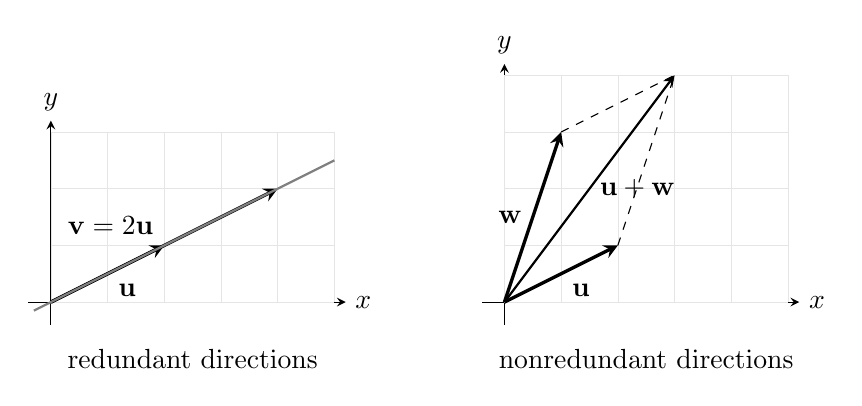
\begin{tikzpicture}[scale=0.72, >=stealth]
    \begin{scope}
        \draw[->] (-0.4,0) -- (5.2,0) node[right] {\(x\)};
        \draw[->] (0,-0.4) -- (0,3.2) node[above] {\(y\)};
        \draw[step=1, gray!20, very thin] (0,0) grid (5,3);

        \draw[->, very thick] (0,0) -- (2,1) node[midway, below right] {\(\mathbf u\)};
        \draw[->, very thick] (0,0) -- (4,2) node[midway, above left] {\(\mathbf v=2\mathbf u\)};
        \draw[thick, gray] (-0.3,-0.15) -- (5,2.5);

        \node at (2.5,-1.0) {redundant directions};
    \end{scope}

    \begin{scope}[xshift=8cm]
        \draw[->] (-0.4,0) -- (5.2,0) node[right] {\(x\)};
        \draw[->] (0,-0.4) -- (0,4.2) node[above] {\(y\)};
        \draw[step=1, gray!20, very thin] (0,0) grid (5,4);

        \draw[->, very thick] (0,0) -- (2,1) node[midway, below right] {\(\mathbf u\)};
        \draw[->, very thick] (0,0) -- (1,3) node[midway, left] {\(\mathbf w\)};
        \draw[dashed] (2,1) -- (3,4);
        \draw[dashed] (1,3) -- (3,4);
        \draw[->, thick] (0,0) -- (3,4) node[midway, right] {\(\mathbf u+\mathbf w\)};

        \node at (2.5,-1.0) {nonredundant directions};
    \end{scope}
\end{tikzpicture}
\caption{Two arrows may be two copies of one direction, or they may give two genuine directions.}
\end{figure}

The equation
\[
    2\mathbf u-\mathbf v=\mathbf 0
\]
reveals the redundancy in the first pair.  It says that a nonzero combination of the
vectors cancels out completely.  That is the key idea.

\begin{definition}[Linear independence]
A list of vectors
\[
    \mathbf v_1,\mathbf v_2,\ldots,\mathbf v_k
\]
is called \emph{linearly independent} if the only way to make
\[
    c_1\mathbf v_1+c_2\mathbf v_2+\cdots+c_k\mathbf v_k=\mathbf 0
\]
is to use
\[
    c_1=c_2=\cdots=c_k=0.
\]
If there is a nonzero choice of coefficients that gives the zero vector, the vectors are
called \emph{linearly dependent}.
\end{definition}

A linear dependence relation is a sign that one direction is unnecessary.  For example,
\[
    2(2,1)-(4,2)=(0,0)
\]
says that \((4,2)\) is already built from \((2,1)\).

A few immediate facts are worth keeping close:

\[
\begin{array}{c|c}
\text{List of vectors} & \text{Independent or dependent?} \\ \hline
\text{one nonzero vector} & \text{independent} \\
\text{any list containing } \mathbf 0 & \text{dependent} \\
\text{two vectors where one is a multiple of the other} & \text{dependent}
\end{array}
\]

The zero vector is always redundant because
\[
    1\cdot \mathbf 0=\mathbf 0
\]
is a nontrivial zero combination.

\subsection{Linear independence in \(\mathbb R^2\) and \(\mathbb R^3\)}

In the plane, the picture is especially simple.

\begin{theorem}[Two directions in the plane]
Two vectors in \(\mathbb R^2\) are linearly independent exactly when neither vector is
a scalar multiple of the other.
\end{theorem}

\begin{proof}[Why this is true]
If one vector is a multiple of the other, say
\[
    \mathbf v=c\mathbf u,
\]
then
\[
    c\mathbf u-\mathbf v=\mathbf 0.
\]
That is a nontrivial zero combination, so the vectors are dependent.

Conversely, suppose two vectors are dependent.  Then there are numbers \(a\) and \(b\),
not both zero, such that
\[
    a\mathbf u+b\mathbf v=\mathbf 0.
\]
If \(b\neq 0\), then
\[
    \mathbf v=-\frac{a}{b}\mathbf u.
\]
So \(\mathbf v\) is a multiple of \(\mathbf u\).  If \(b=0\), then \(a\neq 0\), and the
equation gives \(\mathbf u=\mathbf 0\), which is also a multiple of \(\mathbf v\).
\end{proof}

\begin{example}[Checking independence in the plane]
Let
\[
    \mathbf u=(2,1),\qquad \mathbf w=(1,3).
\]
Suppose
\[
    a\mathbf u+b\mathbf w=\mathbf 0.
\]
Then
\[
    a(2,1)+b(1,3)=(0,0),
\]
so
\[
    (2a+b,\;a+3b)=(0,0).
\]
This gives the system
\[
    2a+b=0,\qquad a+3b=0.
\]
From the first equation,
\[
    b=-2a.
\]
Substitute into the second:
\[
    a+3(-2a)=0,
\]
so
\[
    -5a=0.
\]
Thus \(a=0\), and then \(b=0\).  The only zero combination is the trivial one, so
\(\mathbf u\) and \(\mathbf w\) are linearly independent.
\end{example}

In space, the same idea is present, but the geometry has one more possibility.  Two
nonparallel vectors span a plane through the origin.  A third vector may either leave
that plane or stay inside it.

\begin{example}[Three directions that look like space but are only a plane]
Let
\[
    \mathbf u=(1,0,1),\qquad
    \mathbf v=(0,1,1),\qquad
    \mathbf w=(1,1,2).
\]
These are three vectors in \(\mathbb R^3\).  But
\[
    \mathbf w=\mathbf u+\mathbf v.
\]
Therefore
\[
    \mathbf u+\mathbf v-\mathbf w=\mathbf 0.
\]
This is a nontrivial zero combination, so the three vectors are linearly dependent.
They do not give three independent directions in space.  The third one was already
inside the plane spanned by the first two.
\end{example}

The standard vectors
\[
    \mathbf e_1=(1,0,0),\qquad
    \mathbf e_2=(0,1,0),\qquad
    \mathbf e_3=(0,0,1)
\]
are independent in \(\mathbb R^3\), because
\[
    a\mathbf e_1+b\mathbf e_2+c\mathbf e_3
    =
    (a,b,c).
\]
This is \((0,0,0)\) only when
\[
    a=b=c=0.
\]

\subsection{Bases and coordinates relative to a basis}

The standard basis is not the only possible coordinate system.  On a city map with
diagonal streets, it may be more natural to use diagonal directions.

Let
\[
    \mathbf b_1=(1,1),\qquad
    \mathbf b_2=(1,-1).
\]
These two vectors point along two diagonal directions in the plane.

Suppose a wind displacement is
\[
    \mathbf v=(5,1)
\]
in standard coordinates.  We want to describe the same displacement using
\(\mathbf b_1\) and \(\mathbf b_2\):
\[
    \mathbf v=a\mathbf b_1+b\mathbf b_2.
\]
That means
\[
    (5,1)=a(1,1)+b(1,-1).
\]
So
\[
    (5,1)=(a+b,\;a-b).
\]
Matching components gives
\[
    a+b=5,\qquad a-b=1.
\]
Adding the equations,
\[
    2a=6,
\]
so
\[
    a=3.
\]
Then
\[
    b=2.
\]
Thus
\[
    (5,1)=3(1,1)+2(1,-1).
\]

The vector has standard coordinates \((5,1)\), but relative to the diagonal basis
\[
    \mathcal B=(\mathbf b_1,\mathbf b_2),
\]
its coordinates are
\[
    [\mathbf v]_{\mathcal B}=(3,2).
\]
Those are not a new vector.  They are instructions in a different coordinate language.

\begin{definition}[Basis]
A list of vectors is a \emph{basis} for a space if it satisfies two conditions:

\[
\begin{array}{ll}
\text{1. It spans the space:} & \text{every vector can be built from it.}\\[2mm]
\text{2. It is linearly independent:} & \text{no vector in the list is redundant.}
\end{array}
\]
\end{definition}

When a basis is used for coordinates, the order matters.  The basis
\[
    (\mathbf b_1,\mathbf b_2)
\]
is an ordered list, not just a set.  The first coordinate tells how much of the first
basis vector to use; the second coordinate tells how much of the second basis vector
to use.

\begin{theorem}[Coordinates in a basis]
Let
\[
    \mathcal B=(\mathbf b_1,\mathbf b_2,\ldots,\mathbf b_n)
\]
be a basis for \(\mathbb R^n\).  Then every vector \(\mathbf v\in\mathbb R^n\) has
one and only one expression of the form
\[
    \mathbf v
    =
    c_1\mathbf b_1+c_2\mathbf b_2+\cdots+c_n\mathbf b_n.
\]
The numbers
\[
    c_1,c_2,\ldots,c_n
\]
are called the coordinates of \(\mathbf v\) relative to the basis \(\mathcal B\).
\end{theorem}

\begin{proof}[Why this is true]
Because the basis spans \(\mathbb R^n\), every vector has at least one expression as a
linear combination of the basis vectors.

Now suppose a vector has two such expressions:
\[
    \mathbf v
    =
    c_1\mathbf b_1+\cdots+c_n\mathbf b_n
\]
and
\[
    \mathbf v
    =
    d_1\mathbf b_1+\cdots+d_n\mathbf b_n.
\]
Subtract the second equation from the first:
\[
    \mathbf 0
    =
    (c_1-d_1)\mathbf b_1+\cdots+(c_n-d_n)\mathbf b_n.
\]
Since the basis vectors are linearly independent, the only zero combination is the
trivial one.  Therefore
\[
    c_1-d_1=0,\qquad \ldots,\qquad c_n-d_n=0.
\]
So
\[
    c_1=d_1,\qquad \ldots,\qquad c_n=d_n.
\]
The coordinates are unique.
\end{proof}

Both conditions in the definition of a basis are necessary.

If a list spans but is not independent, coordinates need not be unique.  In
\(\mathbb R^2\), the three vectors
\[
    (1,0),\qquad (0,1),\qquad (1,1)
\]
span the plane, but they are dependent because
\[
    (1,0)+(0,1)-(1,1)=\mathbf 0.
\]
The vector \((1,1)\) has at least two descriptions:
\[
    (1,1)=1(1,1)
\]
and
\[
    (1,1)=1(1,0)+1(0,1).
\]
So spanning alone gives existence, but not uniqueness.

If a list is independent but does not span, some vectors cannot be described at all.
The one-vector list
\[
    (1,0)
\]
is linearly independent in \(\mathbb R^2\), but it does not span the plane.  It can
build only vectors of the form
\[
    a(1,0)=(a,0).
\]
It cannot build \((0,1)\).  So independence alone prevents redundancy, but it does not
guarantee enough directions.

A basis is exactly the balance point: enough directions, but no extra directions.

\subsection{Dimension as the number of independent directions}

A line has one direction.  A plane has two.  Ordinary space has three.  The word
\emph{dimension} makes this counting precise.

\begin{definition}[Dimension]
The \emph{dimension} of a space is the number of vectors in a basis for that space.
\end{definition}

The standard basis of \(\mathbb R^2\) has two vectors:
\[
    (1,0),\qquad (0,1).
\]
So
\[
    \dim(\mathbb R^2)=2.
\]
The standard basis of \(\mathbb R^3\) has three vectors:
\[
    (1,0,0),\qquad (0,1,0),\qquad (0,0,1).
\]
So
\[
    \dim(\mathbb R^3)=3.
\]
In general, the standard basis of \(\mathbb R^n\) has \(n\) vectors, so
\[
    \dim(\mathbb R^n)=n.
\]

Inside a larger space, a span may have smaller dimension.  For example,
\[
    \operatorname{span}\{(2,1,0)\}
\]
is a line through the origin in \(\mathbb R^3\), so it is one-dimensional.

The span
\[
    \operatorname{span}\{(1,0,0),(0,1,0)\}
\]
is the \(xy\)-plane in \(\mathbb R^3\), so it is two-dimensional.

The span
\[
    \operatorname{span}\{(1,0,0),(0,1,0),(0,0,1)\}
\]
is all of \(\mathbb R^3\), so it is three-dimensional.

The dimension counts genuine directions, not the number of vectors written down.  The
three vectors
\[
    (1,0,0),\qquad (0,1,0),\qquad (1,1,0)
\]
span only the \(xy\)-plane, because the third is built from the first two:
\[
    (1,1,0)=(1,0,0)+(0,1,0).
\]
Three vectors are present, but only two independent directions are present.

\subsection{A preview of tangent spaces}

The language of spans, bases, and dimension will return in a new form when we study
curves and surfaces.

A curve has one direction of motion at each point, as long as it is not stopped there.
For example, the curve
\[
    \mathbf r(t)=(t,t^2)
\]
passes through
\[
    \mathbf r(1)=(1,1).
\]
Its velocity is
\[
    \mathbf r'(t)=(1,2t),
\]
so at \(t=1\),
\[
    \mathbf r'(1)=(1,2).
\]
The tangent line at \((1,1)\) has the form
\[
    (1,1)+s(1,2).
\]
That is an affine line: a point plus the span of one direction.

A surface usually has two independent tangent directions at each point.  Those two
directions span a tangent plane.  Later, when we differentiate parametrized surfaces,
this idea will become concrete:
\[
    \text{tangent plane}=\text{point}+\operatorname{span}\{\text{two tangent directions}\}.
\]

This is the first glimpse of a theme that will follow us through the book.  Geometry
near a point often becomes linear.  A curve becomes a tangent line.  A surface becomes
a tangent plane.  A nonlinear function becomes its best linear approximation.

Linear independence tells us when directions can serve as coordinates.  But it does
not yet tell us how long a direction is.  In standard coordinates the vector \((3,4)\)
has length \(5\), but in a diagonal or slanted basis the coordinate pair \((3,4)\) may
represent a very different geometric arrow.  To talk about speed, distance, spheres, and
unit directions, we need a way to measure length itself.
\section{Norm, distance, and spheres}

The last section ended with a simple problem.  We know how to describe directions with
vectors, and we know when directions are redundant.  But we still do not know how long
a vector is.

That question sounds small.  It is not.  Length is what turns a displacement into a
distance, a velocity vector into a speed, and a direction into a unit direction.

\subsection{Length of a vector}

A drone receives the command
\[
    \mathbf v=(6,2,3).
\]
The command means:
\[
    6 \text{ meters east},\qquad 2 \text{ meters north},\qquad 3 \text{ meters up}.
\]
How far is the drone from where it started?

First ignore the upward motion.  On the floor, the drone moves
\[
    (6,2),
\]
whose length is
\[
    \sqrt{6^2+2^2}=\sqrt{40}.
\]
Now add the upward motion.  The floor displacement \(\sqrt{40}\) and the height \(3\)
make another right triangle, so the total length is
\[
    \sqrt{(\sqrt{40})^2+3^2}
    =
    \sqrt{40+9}
    =
    7.
\]
The vector \((6,2,3)\) has length \(7\).

\begin{definition}[Norm]
The \emph{norm} of a vector
\[
    \mathbf v=(v_1,v_2,\ldots,v_n)
\]
in \(\mathbb R^n\) is
\[
    \|\mathbf v\|
    =
    \sqrt{v_1^2+v_2^2+\cdots+v_n^2}.
\]
The norm is also called the \emph{length} or \emph{magnitude} of the vector.
\end{definition}

In the plane,
\[
    \|(a,b)\|=\sqrt{a^2+b^2}.
\]
In space,
\[
    \|(a,b,c)\|=\sqrt{a^2+b^2+c^2}.
\]

\begin{example}[A familiar length]
The vector
\[
    \mathbf v=(3,4)
\]
has norm
\[
    \|\mathbf v\|=\sqrt{3^2+4^2}=5.
\]
So the old \(3\)-\(4\)-\(5\) right triangle is now a vector length calculation.
\end{example}

\begin{example}[A space displacement]
The vector
\[
    \mathbf w=(2,-1,2)
\]
has norm
\[
    \|\mathbf w\|
    =
    \sqrt{2^2+(-1)^2+2^2}
    =
    \sqrt{9}
    =
    3.
\]
The negative sign does not make the vector shorter or longer.  It only says that the
motion in that coordinate direction is opposite to the positive direction.
\end{example}

\begin{figure}[h]
\centering
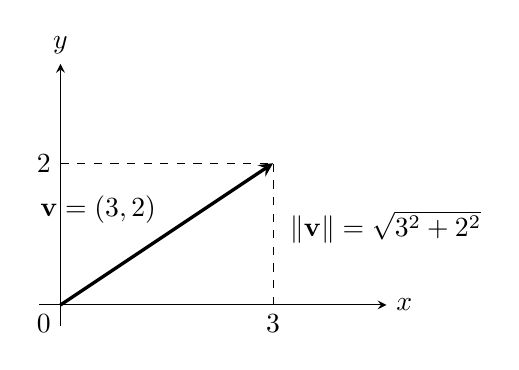
\begin{tikzpicture}[scale=0.9, >=stealth]
    \draw[->] (-0.3,0) -- (4.6,0) node[right] {\(x\)};
    \draw[->] (0,-0.3) -- (0,3.4) node[above] {\(y\)};

    \draw[->, very thick] (0,0) -- (3,2) node[midway, above left] {\(\mathbf v=(3,2)\)};
    \draw[dashed] (3,0) -- (3,2);
    \draw[dashed] (0,2) -- (3,2);

    \node[below] at (3,0) {\(3\)};
    \node[left] at (0,2) {\(2\)};
    \node[below left] at (0,0) {\(0\)};

    \node[right] at (3.1,1.1) {\(\|\mathbf v\|=\sqrt{3^2+2^2}\)};
\end{tikzpicture}
\caption{The norm is the distance from the tail of the vector to its head.}
\end{figure}

The norm of the zero vector is
\[
    \|\mathbf 0\|=0.
\]
Every other vector has positive norm.

\subsection{Distance between points}

A vector has length.  Two points have distance between them.

Suppose a ranger station is at
\[
    P=(2,1)
\]
on a map, and a campfire is reported at
\[
    Q=(8,9).
\]
The displacement from \(P\) to \(Q\) is
\[
    Q-P=(8-2,\;9-1)=(6,8).
\]
Therefore the distance from \(P\) to \(Q\) is
\[
    \|Q-P\|
    =
    \|(6,8)\|
    =
    \sqrt{6^2+8^2}
    =
    10.
\]

\begin{definition}[Distance]
The distance between points
\[
    P=(p_1,p_2,\ldots,p_n)
\]
and
\[
    Q=(q_1,q_2,\ldots,q_n)
\]
in \(\mathbb R^n\) is
\[
    d(P,Q)
    =
    \|Q-P\|
    =
    \sqrt{(q_1-p_1)^2+(q_2-p_2)^2+\cdots+(q_n-p_n)^2}.
\]
\end{definition}

The order of the points does not matter:
\[
    d(P,Q)=d(Q,P).
\]
Indeed,
\[
    Q-P=-(P-Q),
\]
and a vector and its negative have the same length.

\begin{example}[Distance in space]
Let
\[
    P=(1,2,0),\qquad Q=(4,-2,12).
\]
Then
\[
    Q-P=(3,-4,12),
\]
so
\[
    d(P,Q)
    =
    \sqrt{3^2+(-4)^2+12^2}
    =
    \sqrt{9+16+144}
    =
    13.
\]
\end{example}

Notice the pattern:

\[
\begin{array}{c|c}
\text{Object} & \text{What we measure} \\ \hline
\mathbf v & \|\mathbf v\| \\
P,Q & d(P,Q)=\|Q-P\|
\end{array}
\]

A vector has a length by itself.  Two points have a distance because their difference is
a vector.

\subsection{Circles, spheres, and higher-dimensional spheres}

A radio transmitter sits at
\[
    C=(3,2)
\]
on a flat map.  Its signal reaches every point within \(5\) km of \(C\).  The edge of the
coverage region is the set of points \((x,y)\) whose distance from \(C\) is \(5\):
\[
    d((x,y),C)=5.
\]
Using the distance formula,
\[
    \sqrt{(x-3)^2+(y-2)^2}=5.
\]
Squaring both sides gives
\[
    (x-3)^2+(y-2)^2=25.
\]
This is a circle.

The filled-in coverage region is
\[
    (x-3)^2+(y-2)^2\leq 25.
\]
The boundary is a circle; the filled-in region is a disk.

\begin{figure}[h]
\centering
\begin{tikzpicture}[scale=0.75, >=stealth]
    \draw[->] (-2,0) -- (9,0) node[right] {\(x\)};
    \draw[->] (0,-3) -- (0,8) node[above] {\(y\)};

    \draw[thick] (3,2) circle (3.2);
    \fill (3,2) circle (2pt);
    \node[below left] at (3,2) {\(C=(3,2)\)};

    \draw[->, thick] (3,2) -- (6.2,2);
    \node[above] at (4.7,2) {\(5\)};

    \node at (3,-2.0) {\((x-3)^2+(y-2)^2=25\)};
\end{tikzpicture}
\caption{A circle is the set of points at a fixed distance from a center.}
\end{figure}

The same idea works in space.  A point \((x,y,z)\) is on the sphere of radius \(5\)
centered at
\[
    C=(3,2,1)
\]
when
\[
    d((x,y,z),C)=5.
\]
Thus
\[
    (x-3)^2+(y-2)^2+(z-1)^2=25.
\]

\begin{definition}[Spheres and balls]
In \(\mathbb R^n\), the sphere of radius \(r\geq 0\) centered at
\[
    C=(c_1,c_2,\ldots,c_n)
\]
is the set of points \(X=(x_1,x_2,\ldots,x_n)\) satisfying
\[
    \|X-C\|=r.
\]
Equivalently,
\[
    (x_1-c_1)^2+(x_2-c_2)^2+\cdots+(x_n-c_n)^2=r^2.
\]

The ball of radius \(r\) centered at \(C\) is the set of points satisfying
\[
    \|X-C\|\leq r.
\]
\end{definition}

In \(\mathbb R^2\), a sphere is what we usually call a circle.  In \(\mathbb R^3\), a
sphere is the surface of a round ball.  In \(\mathbb R^4\) and beyond, we cannot draw
the sphere honestly, but the equation still makes perfect sense.

The condition \(r\geq 0\) is not decoration.  Distance is never negative.  If \(r<0\),
then
\[
    \|X-C\|=r
\]
has no solutions.  If \(r=0\), the sphere is just the single point \(C\).

\subsection{The triangle inequality and why it matters}

A hiker walks from a cabin to a lake, then from the lake to a lookout point.  The direct
path from the cabin to the lookout cannot be longer than the broken path through the
lake.  This everyday fact becomes one of the most useful inequalities in calculus.

For example, let
\[
    \mathbf u=(3,1),\qquad \mathbf v=(1,2).
\]
Then
\[
    \mathbf u+\mathbf v=(4,3).
\]
The lengths are
\[
    \|\mathbf u\|=\sqrt{10},\qquad
    \|\mathbf v\|=\sqrt{5},\qquad
    \|\mathbf u+\mathbf v\|=5.
\]
The direct vector \(\mathbf u+\mathbf v\) is shorter than taking \(\mathbf u\) and then
\(\mathbf v\):
\[
    5
    \leq
    \sqrt{10}+\sqrt{5}.
\]

\begin{theorem}[Triangle inequality]
For any vectors \(\mathbf u,\mathbf v\in\mathbb R^n\),
\[
    \|\mathbf u+\mathbf v\|
    \leq
    \|\mathbf u\|+\|\mathbf v\|.
\]
Equivalently, for any three points \(P,Q,R\in\mathbb R^n\),
\[
    d(P,R)\leq d(P,Q)+d(Q,R).
\]
\end{theorem}

\begin{proof}[Why this is true geometrically]
Draw \(\mathbf u\) first, then draw \(\mathbf v\) starting at the head of \(\mathbf u\).
The vector \(\mathbf u+\mathbf v\) goes directly from the first tail to the last head.
These three segments form a triangle, possibly flattened into a line.  The direct side
of a triangle is never longer than the other two sides together.

A fully algebraic proof will come naturally after the next chapter gives a name to the
expression
\[
    u_1v_1+u_2v_2+\cdots+u_nv_n.
\]
That name is the \emph{dot product}.
\end{proof}

Equality happens when the two vectors point in the same direction.  For example,
\[
    \mathbf u=(2,1),\qquad \mathbf v=(6,3)=3\mathbf u.
\]
Then
\[
    \|\mathbf u+\mathbf v\|
    =
    \|(8,4)\|
    =
    4\sqrt{5},
\]
while
\[
    \|\mathbf u\|+\|\mathbf v\|
    =
    \sqrt5+3\sqrt5
    =
    4\sqrt5.
\]
The broken path is not really broken; both pieces lie along the same ray.

The triangle inequality will return often.  When we later say that a function is
continuous, or that a curve stays close to another curve, the triangle inequality is the
tool that lets us control a complicated distance by breaking it into simpler pieces.

\subsection{Unit vectors and normalization}

Sometimes length is not what we care about.  We only want direction.

A wind sensor reports the displacement direction
\[
    \mathbf v=(6,2).
\]
Its length is
\[
    \|\mathbf v\|=\sqrt{6^2+2^2}=\sqrt{40}=2\sqrt{10}.
\]
If we divide \(\mathbf v\) by its own length, we get
\[
    \frac{\mathbf v}{\|\mathbf v\|}
    =
    \frac{(6,2)}{2\sqrt{10}}
    =
    \left(\frac{3}{\sqrt{10}},\frac{1}{\sqrt{10}}\right).
\]
This new vector points in the same direction as \(\mathbf v\), but has length \(1\).

\begin{definition}[Unit vector and normalization]
A vector \(\mathbf u\) is a \emph{unit vector} if
\[
    \|\mathbf u\|=1.
\]
If \(\mathbf v\neq \mathbf 0\), the unit vector in the direction of \(\mathbf v\) is
\[
    \widehat{\mathbf v}
    =
    \frac{\mathbf v}{\|\mathbf v\|}.
\]
This process is called \emph{normalizing} the vector.
\end{definition}

The condition \(\mathbf v\neq \mathbf 0\) matters.  The formula
\[
    \frac{\mathbf v}{\|\mathbf v\|}
\]
would require division by \(0\) if \(\mathbf v=\mathbf 0\).  But the deeper problem is
geometric: the zero vector has no direction.  There is no unit vector pointing in the
same direction as no direction.

\begin{example}[Speed and direction]
A small boat has velocity
\[
    \mathbf v=(12,5)
\]
measured in meters per second.  Its speed is
\[
    \|\mathbf v\|=\sqrt{12^2+5^2}=13.
\]
Its direction is the unit vector
\[
    \widehat{\mathbf v}
    =
    \left(\frac{12}{13},\frac{5}{13}\right).
\]
So the velocity can be written as
\[
    \mathbf v
    =
    13\left(\frac{12}{13},\frac{5}{13}\right).
\]
This separates the motion into
\[
    \text{speed}\times\text{direction}.
\]
\end{example}

Now that length and distance are available, our earlier descriptions of lines and planes
become sharper.  A road is not just a set of points of the form \(P+t\mathbf u\); we can
ask how far a house is from that road.  A wall is not just a flat surface; we can ask for
the shortest distance from a sensor to the wall.  Those questions lead us back to lines
and planes, but now with measurement attached.

\section{Lines, planes, and hyperplanes}

In \S1.2, lines and planes appeared as translated spans:
\[
    P+\operatorname{span}\{\mathbf u\},
    \qquad
    P+\operatorname{span}\{\mathbf u,\mathbf v\}.
\]
In \S1.5, we learned how to measure distance.  Put those together, and flat geometry
becomes useful: we can describe roads, walls, flight paths, and constraints, and then
measure how far away things are from them.

\subsection{Parametric equations of lines}

A trail in space begins at
\[
    P=(2,-1,3)
\]
and follows the direction
\[
    \mathbf u=(1,4,-2).
\]
A point on the trail has the form
\[
    P+t\mathbf u
    =
    (2,-1,3)+t(1,4,-2).
\]
Writing the coordinates separately gives
\[
    x=2+t,\qquad y=-1+4t,\qquad z=3-2t.
\]
The parameter \(t\) tells how far we have moved in the chosen direction, measured in
units of the vector \(\mathbf u\).

\begin{definition}[Parametric equation of a line]
Let \(P\) be a point in \(\mathbb R^n\), and let \(\mathbf u\neq \mathbf 0\) be a vector.
The line through \(P\) in the direction \(\mathbf u\) is
\[
    L=\{P+t\mathbf u:t\in\mathbb R\}.
\]
The equation
\[
    X=P+t\mathbf u
\]
is called a \emph{parametric equation} of the line.
\end{definition}

The condition \(\mathbf u\neq \mathbf 0\) is essential.  If \(\mathbf u=\mathbf 0\), then
\[
    P+t\mathbf 0=P
\]
for every \(t\).  The formula does not trace a line at all.  It stays at one point.

\begin{example}[A line in the plane]
The line through
\[
    P=(1,2)
\]
in the direction
\[
    \mathbf u=(3,1)
\]
has parametric equation
\[
    (x,y)=(1,2)+t(3,1).
\]
Thus
\[
    x=1+3t,\qquad y=2+t.
\]
When \(t=0\), the point is \((1,2)\).  When \(t=2\), the point is
\[
    (1,2)+2(3,1)=(7,4).
\]
When \(t=-1\), the point is
\[
    (1,2)-(3,1)=(-2,1).
\]
\end{example}

The same geometric line can have many parametric equations.  For example,
\[
    (x,y)=(1,2)+t(3,1)
\]
and
\[
    (x,y)=(7,4)+s(-6,-2)
\]
describe the same line.  The second one starts at a different point and uses a direction
vector pointing the opposite way with twice the length.

A parametrization is a way of moving through the line, not the line itself.

\subsection{Parametric equations of planes}

A flat sheet in space needs a point and two independent directions.

Suppose a shade sail has one corner at
\[
    P=(1,0,2)
\]
and follows two support directions
\[
    \mathbf u=(2,1,0),\qquad
    \mathbf v=(0,1,3).
\]
Points on the sail have the form
\[
    P+s\mathbf u+t\mathbf v.
\]
So
\[
    (x,y,z)
    =
    (1,0,2)+s(2,1,0)+t(0,1,3),
\]
or
\[
    x=1+2s,\qquad y=s+t,\qquad z=2+3t.
\]

\begin{definition}[Parametric equation of a plane]
Let \(P\) be a point in \(\mathbb R^3\), and let \(\mathbf u\) and \(\mathbf v\) be two
vectors that are not scalar multiples of each other.  The plane through \(P\) in the
directions \(\mathbf u\) and \(\mathbf v\) is
\[
    \Pi
    =
    \{P+s\mathbf u+t\mathbf v:s,t\in\mathbb R\}.
\]
The equation
\[
    X=P+s\mathbf u+t\mathbf v
\]
is called a \emph{parametric equation} of the plane.
\end{definition}

The condition on \(\mathbf u\) and \(\mathbf v\) matters.  If
\[
    \mathbf v=3\mathbf u,
\]
then
\[
    P+s\mathbf u+t\mathbf v
    =
    P+s\mathbf u+3t\mathbf u
    =
    P+(s+3t)\mathbf u.
\]
This is only a line.  Two written vectors do not guarantee two genuine directions.

\begin{figure}[h]
\centering
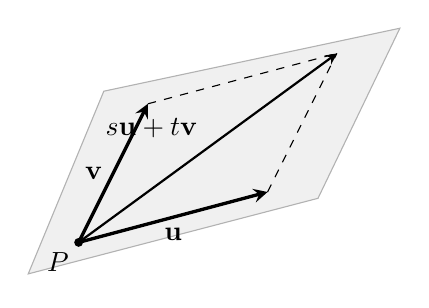
\begin{tikzpicture}[scale=0.8, >=stealth]
    \coordinate (P) at (0,0);
    \coordinate (U) at (3,0.8);
    \coordinate (V) at (1.1,2.2);
    \coordinate (UV) at (4.1,3.0);

    \filldraw[fill=gray!12, draw=gray!60] (-0.8,-0.5) -- (3.8,0.7) -- (5.1,3.4) -- (0.4,2.4) -- cycle;

    \draw[->, very thick] (P) -- (U) node[midway, below] {\(\mathbf u\)};
    \draw[->, very thick] (P) -- (V) node[midway, left] {\(\mathbf v\)};
    \draw[->, thick] (P) -- (UV) node[midway, above left] {\(s\mathbf u+t\mathbf v\)};

    \draw[dashed] (U) -- (UV);
    \draw[dashed] (V) -- (UV);

    \fill (P) circle (2pt);
    \node[below left] at (P) {\(P\)};
\end{tikzpicture}
\caption{A plane is swept out by two independent directions from a starting point.}
\end{figure}

\subsection{Normal equations of planes}

Parametric equations describe how to move around inside a plane.  There is another
way to describe a plane: give a direction straight across it.

Consider the plane
\[
    2x-y+3z=0.
\]
If we move inside this plane by a small displacement
\[
    (\Delta x,\Delta y,\Delta z),
\]
then the value of \(2x-y+3z\) should not change.  Therefore the displacement must
satisfy
\[
    2\Delta x-\Delta y+3\Delta z=0.
\]
For example,
\[
    (1,2,0)
\]
is allowed because
\[
    2(1)-2+3(0)=0.
\]
Also
\[
    (0,3,1)
\]
is allowed because
\[
    2(0)-3+3(1)=0.
\]
These are directions along the plane.

The coefficients
\[
    (2,-1,3)
\]
measure motion across the plane.  This vector is called a normal vector to the plane.
The next chapter will explain this language using the dot product.  For now, the key
point is that the plane is made of all points where the linear expression
\[
    2x-y+3z
\]
has one fixed value.

\begin{definition}[Normal equation of a plane]
Let
\[
    \mathbf n=(A,B,C)\neq \mathbf 0
\]
and let
\[
    P_0=(x_0,y_0,z_0).
\]
The plane through \(P_0\) with normal vector \(\mathbf n\) has equation
\[
    A(x-x_0)+B(y-y_0)+C(z-z_0)=0.
\]
Equivalently, it can be written
\[
    Ax+By+Cz=D
\]
for some constant \(D\).
\end{definition}

The condition
\[
    (A,B,C)\neq (0,0,0)
\]
is necessary.  If \(A=B=C=0\), then the equation becomes
\[
    0=D.
\]
If \(D=0\), every point in space satisfies it.  If \(D\neq0\), no point satisfies it.
Neither case gives a plane.

\begin{example}[From a normal vector to a plane equation]
Find the plane through
\[
    P_0=(1,2,0)
\]
with normal vector
\[
    \mathbf n=(2,-1,3).
\]
Using the definition,
\[
    2(x-1)-(y-2)+3(z-0)=0.
\]
Simplifying,
\[
    2x-2-y+2+3z=0,
\]
so
\[
    2x-y+3z=0.
\]
\end{example}

\begin{example}[From a plane equation to a parametrization]
The plane
\[
    2x-y+3z=0
\]
can be parametrized by choosing two coordinates freely.  Let
\[
    x=s,\qquad z=t.
\]
Then the equation gives
\[
    2s-y+3t=0,
\]
so
\[
    y=2s+3t.
\]
Therefore
\[
    (x,y,z)=(s,2s+3t,t).
\]
Writing this as a point plus directions,
\[
    (x,y,z)
    =
    s(1,2,0)+t(0,3,1).
\]
So a parametric equation is
\[
    (x,y,z)=s(1,2,0)+t(0,3,1).
\]
\end{example}

The two descriptions tell different stories.

\[
\begin{array}{c|c}
\text{Parametric equation} & \text{How to move inside the plane} \\
\text{Normal equation} & \text{How to test whether a point is on the plane}
\end{array}
\]

Both are useful.

\subsection{Distances to lines and planes}

Distance questions turn flat geometry into calculus.

A road in the plane is described by
\[
    L=(1,2)+t(3,1).
\]
A house is located at
\[
    A=(4,6).
\]
How far is the house from the road?

A point on the road is
\[
    P(t)=(1+3t,\;2+t).
\]
The squared distance from \(A\) to \(P(t)\) is
\[
\begin{aligned}
    D(t)^2
    &=
    (4-(1+3t))^2+(6-(2+t))^2  \\
    &=
    (3-3t)^2+(4-t)^2.
\end{aligned}
\]
We minimize \(D(t)^2\) instead of \(D(t)\), because the square root is not needed to
find the closest point.

Expanding,
\[
    D(t)^2=10t^2-26t+25.
\]
This is a single-variable calculus problem.  Differentiate:
\[
    \frac{d}{dt}D(t)^2=20t-26.
\]
Set this equal to zero:
\[
    20t-26=0,
\]
so
\[
    t=\frac{13}{10}.
\]
The nearest point on the road is
\[
    P\left(\frac{13}{10}\right)
    =
    \left(1+3\cdot\frac{13}{10},\;2+\frac{13}{10}\right)
    =
    \left(\frac{49}{10},\frac{33}{10}\right).
\]
The distance is
\[
\begin{aligned}
    d(A,L)
    &=
    \sqrt{\left(4-\frac{49}{10}\right)^2+
          \left(6-\frac{33}{10}\right)^2}  \\
    &=
    \sqrt{\left(-\frac{9}{10}\right)^2+
          \left(\frac{27}{10}\right)^2} \\
    &=
    \frac{9\sqrt{10}}{10}.
\end{aligned}
\]

\begin{example}[The nearest point formula for a line]
Let
\[
    L=P+t\mathbf u
\]
be a line in \(\mathbb R^n\), where
\[
    P=(p_1,\ldots,p_n),\qquad
    \mathbf u=(u_1,\ldots,u_n)\neq \mathbf 0.
\]
Let
\[
    A=(a_1,\ldots,a_n)
\]
be a point.

The value of \(t\) that gives the closest point on the line is
\[
    t_*
    =
    \frac{(a_1-p_1)u_1+\cdots+(a_n-p_n)u_n}
         {u_1^2+\cdots+u_n^2}.
\]
Then the distance from \(A\) to the line is
\[
    d(A,L)=\|A-(P+t_*\mathbf u)\|.
\]
The numerator in this formula will soon get a name.  It is the dot product hiding in
plain sight.
\end{example}

Planes have an especially clean distance formula.

\begin{example}[Distance from a point to a plane]
Find the distance from
\[
    A=(3,1,4)
\]
to the plane
\[
    2x-y+2z=5.
\]
The normal direction is
\[
    \mathbf n=(2,-1,2).
\]
A line starting at \(A\) and moving straight across the plane is
\[
    (x,y,z)=(3,1,4)+t(2,-1,2).
\]
Substitute this into the plane equation:
\[
    2(3+2t)-(1-t)+2(4+2t)=5.
\]
Simplify:
\[
    13+9t=5.
\]
Thus
\[
    t=-\frac{8}{9}.
\]
The distance traveled along the normal line is
\[
    \left|-\frac{8}{9}\right|\|(2,-1,2)\|
    =
    \frac{8}{9}\sqrt{4+1+4}
    =
    \frac{8}{3}.
\]
So the distance from the point to the plane is
\[
    \frac83.
\]
\end{example}

\begin{theorem}[Distance from a point to a plane]
Let
\[
    \Pi:\quad \alpha x+\beta y+\gamma z=d
\]
be a plane, where
\[
    (\alpha,\beta,\gamma)\neq (0,0,0).
\]
The distance from
\[
    A=(a,b,c)
\]
to \(\Pi\) is
\[
    \boxed{
    d(A,\Pi)
    =
    \frac{|\alpha a+\beta b+\gamma c-d|}
         {\sqrt{\alpha^2+\beta^2+\gamma^2}}.
    }
\]
\end{theorem}

\begin{proof}
Move from \(A\) in the normal direction
\[
    \mathbf n=(\alpha,\beta,\gamma).
\]
The normal line is
\[
    (x,y,z)=(a,b,c)+t(\alpha,\beta,\gamma).
\]
Substitute into the plane equation:
\[
    \alpha(a+t\alpha)+\beta(b+t\beta)+\gamma(c+t\gamma)=d.
\]
This becomes
\[
    \alpha a+\beta b+\gamma c
    +
    t(\alpha^2+\beta^2+\gamma^2)
    =
    d.
\]
Thus
\[
    t=
    \frac{d-(\alpha a+\beta b+\gamma c)}
         {\alpha^2+\beta^2+\gamma^2}.
\]
The distance traveled is
\[
    |t|\|\mathbf n\|
    =
    \left|
    \frac{d-(\alpha a+\beta b+\gamma c)}
         {\alpha^2+\beta^2+\gamma^2}
    \right|
    \sqrt{\alpha^2+\beta^2+\gamma^2}.
\]
After simplifying, this gives
\[
    d(A,\Pi)
    =
    \frac{|\alpha a+\beta b+\gamma c-d|}
         {\sqrt{\alpha^2+\beta^2+\gamma^2}}.
\]
\end{proof}

The absolute value is important.  The expression
\[
    \alpha a+\beta b+\gamma c-d
\]
can be positive or negative depending on which side of the plane the point lies.  Distance
does not remember the side.  It only remembers how far.

\subsection{Hyperplanes in \(\mathbb R^n\)}

In \(\mathbb R^2\), an equation like
\[
    3x-2y=5
\]
describes a line.

In \(\mathbb R^3\), an equation like
\[
    3x-2y+z=5
\]
describes a plane.

In \(\mathbb R^4\), an equation like
\[
    3x_1-2x_2+x_3+7x_4=5
\]
describes something we cannot draw honestly.  But the pattern is clear: one linear
constraint removes one free direction.

\begin{definition}[Hyperplane]
A \emph{hyperplane} in \(\mathbb R^n\) is a set of points satisfying one linear equation
\[
    a_1x_1+a_2x_2+\cdots+a_nx_n=d,
\]
where at least one coefficient \(a_i\) is nonzero.
\end{definition}

A hyperplane in \(\mathbb R^2\) is a line.  A hyperplane in \(\mathbb R^3\) is a plane.
A hyperplane in \(\mathbb R^4\) is a three-dimensional flat slice of four-dimensional
space.

\begin{example}[A constraint in a data space]
A greenhouse sensor records four quantities:
\[
    (T,p,h,c),
\]
where \(T\) is temperature, \(p\) is pressure, \(h\) is humidity, and \(c\) is carbon dioxide
level.

Suppose an alarm triggers when
\[
    2T+p-3h+4c=100.
\]
The set of all readings that trigger the alarm is a hyperplane in \(\mathbb R^4\).
We cannot draw it as a surface in ordinary space, but we can still work with it
algebraically.
\end{example}

If
\[
    a_n\neq0,
\]
then the hyperplane equation can be solved for \(x_n\):
\[
    x_n
    =
    \frac{d-a_1x_1-\cdots-a_{n-1}x_{n-1}}{a_n}.
\]
The first \(n-1\) coordinates may be chosen freely, and the last one is then determined.
That is why a hyperplane in \(\mathbb R^n\) has dimension \(n-1\).

Lines, planes, and hyperplanes are the flat objects of multivariable calculus.  They are
simple enough to compute with, but rich enough to approximate curved objects.  Later,
a curve will become a tangent line when we zoom in.  A surface will become a tangent
plane.  A nonlinear constraint will become a hyperplane.

But one important piece is still missing.  We can add vectors and stretch them.  We can
measure their length.  We still cannot multiply two vectors in a useful way.  There is
not just one useful multiplication.  One product will measure how much two directions
agree.  Another will measure the signed area they create.  Those two ideas begin the
next chapter.

\section{Chapter review and discovery problems}

Chapter 1 began with locations and displacements.  It ended with distances to planes
and hyperplanes.  The main change was not a new formula; it was a new way to see
geometry.  Points tell us where.  Vectors tell us how to move.  Spans tell us what
directions can build.  Norms and distances tell us how large those motions are.

The problems below are meant to make those ideas usable.  Some are short checks.
Some are small discoveries.  Draw pictures whenever a picture is possible.

\subsection{Concept check: vectors as objects, not just coordinates}

\begin{enumerate}
    \item What is the difference between a point and a vector, even when both are written
    with ordered pairs such as \((3,4)\)?

    \item Explain why the displacement from
    \[
        P=(2,-1,5)
    \]
    to
    \[
        Q=(7,3,1)
    \]
    is not the point \(Q\), but the vector \(Q-P\).

    \item The same vector can be drawn with its tail at many different points.  Why does
    moving the drawing of an arrow not change the vector it represents?

    \item What does it mean for a vector to be a linear combination of two other vectors?

    \item Why do the vectors
    \[
        (2,1),\qquad (4,2)
    \]
    not give two genuine directions?

    \item Give an example of two vectors in \(\mathbb R^2\) that are linearly independent.
    Explain how you know.

    \item Give an example of three vectors in \(\mathbb R^3\) that are linearly dependent
    even though none of them is the zero vector.

    \item What two conditions must a list of vectors satisfy to be a basis?

    \item Why can the zero vector not be normalized?

    \item What is the difference between the sphere
    \[
        (x-1)^2+(y+2)^2=9
    \]
    and the ball
    \[
        (x-1)^2+(y+2)^2\leq 9?
    \]

    \item A plane can be described parametrically or by a normal equation.  What does
    each description make easy to do?

    \item Why is the equation
    \[
        0x+0y+0z=4
    \]
    not the equation of a plane?
\end{enumerate}

\subsection{Skills: vectors, distances, lines, and planes}

\begin{enumerate}
    \item Let
    \[
        \mathbf u=(3,-1,4),\qquad \mathbf v=(-2,5,0).
    \]
    Compute
    \[
        \mathbf u+\mathbf v,\qquad
        2\mathbf u-3\mathbf v,\qquad
        -\mathbf u.
    \]

    \item Find the norm of each vector:
    \[
        (5,12),\qquad
        (2,-1,2),\qquad
        (1,1,1,1).
    \]

    \item Find the distance between
    \[
        P=(1,2,3)
    \]
    and
    \[
        Q=(5,-1,9).
    \]

    \item Find the equation of the sphere centered at
    \[
        C=(2,-1,4)
    \]
    with radius \(6\).

    \item Find the center and radius of the sphere
    \[
        (x-3)^2+y^2+(z+5)^2=49.
    \]

    \item Normalize the vector
    \[
        \mathbf v=(4,0,-3).
    \]

    \item Write a parametric equation of the line through
    \[
        P=(1,0,2)
    \]
    in the direction
    \[
        \mathbf u=(3,-1,4).
    \]

    \item Does the point
    \[
        (7,-2,10)
    \]
    lie on the line
    \[
        (x,y,z)=(1,0,2)+t(3,-1,4)?
    \]

    \item Write a parametric equation of the plane through
    \[
        P=(0,1,2)
    \]
    in the directions
    \[
        \mathbf u=(1,0,3),\qquad
        \mathbf v=(2,1,0).
    \]

    \item Find three points on the plane
    \[
        (x,y,z)=(0,1,2)+s(1,0,3)+t(2,1,0).
    \]

    \item Find a normal equation for the plane through
    \[
        P_0=(1,2,3)
    \]
    with normal vector
    \[
        \mathbf n=(2,-1,5).
    \]

    \item Does the point
    \[
        (3,4,1)
    \]
    lie on the plane
    \[
        2x-y+5z=9?
    \]

    \item Parametrize the plane
    \[
        x+2y-z=4
    \]
    by choosing \(y=s\) and \(z=t\).

    \item Find the distance from
    \[
        A=(1,2,3)
    \]
    to the plane
    \[
        2x-y+2z=7.
    \]

    \item Find the closest point on the line
    \[
        L=(0,0)+t(2,1)
    \]
    to the point
    \[
        A=(3,4).
    \]
    Then find the distance from \(A\) to \(L\).
\end{enumerate}

\subsection{Discovery: why two independent directions make a plane}

These problems are meant to be explored slowly.  They explain why linear independence
is not just a definition, but the hidden rule behind coordinates.

\begin{enumerate}
    \item Let
    \[
        \mathbf u=(2,1),\qquad
        \mathbf v=(1,3).
    \]
    Try to solve
    \[
        s\mathbf u+t\mathbf v=(x,y)
    \]
    for \(s\) and \(t\).  Your answer should express \(s\) and \(t\) in terms of \(x\)
    and \(y\).  What does this prove about the span of \(\mathbf u\) and \(\mathbf v\)?

    \item Repeat the previous problem with
    \[
        \mathbf u=(2,1),\qquad
        \mathbf v=(4,2).
    \]
    Which points \((x,y)\) can be reached?  Which cannot?

    \item In \(\mathbb R^3\), let
    \[
        \mathbf u=(1,0,1),\qquad
        \mathbf v=(0,1,1).
    \]
    Points in the span of \(\mathbf u\) and \(\mathbf v\) have the form
    \[
        s(1,0,1)+t(0,1,1).
    \]
    Write the coordinates of such a point as \((x,y,z)\).  Then find one equation
    involving \(x,y,z\) that every such point satisfies.

    \item The previous problem found a plane through the origin.  Translate it through
    the point
    \[
        P=(2,0,1).
    \]
    Write both a parametric equation and a normal equation for the translated plane.

    \item Suppose three vectors in \(\mathbb R^3\) all lie in the same plane through the
    origin.  Explain why they must be linearly dependent.

    \item Suppose three vectors in \(\mathbb R^3\) are linearly independent.  Explain why
    they cannot all lie in one plane through the origin.

    \item A basis in \(\mathbb R^2\) is like a pair of street directions.  Use the basis
    \[
        \mathbf b_1=(1,1),\qquad
        \mathbf b_2=(1,-1)
    \]
    to express each vector below in \(\mathcal B\)-coordinates:
    \[
        (4,0),\qquad
        (0,6),\qquad
        (5,1).
    \]

    \item Draw the grid formed by all points
    \[
        s(1,1)+t(1,-1)
    \]
    where \(s\) and \(t\) are integers between \(-3\) and \(3\).  How does this grid
    differ from the usual square coordinate grid?
\end{enumerate}

\subsection{Hook: the need for a multiplication of vectors}

Addition and scaling have carried us far.  But many geometric questions do not ask
for another vector of the same kind.

\begin{enumerate}
    \item A force
    \[
        \mathbf F=(10,0)
    \]
    pushes an object through the displacement
    \[
        \mathbf d=(3,0).
    \]
    It seems natural that the work should be \(30\).  What should the work be if
    \[
        \mathbf d=(0,3)?
    \]
    What about
    \[
        \mathbf d=(3,4)?
    \]
    What kind of vector multiplication would answer this?

    \item The vectors
    \[
        \mathbf u=(3,0),\qquad \mathbf v=(0,2)
    \]
    form a rectangle of area \(6\).  The vectors
    \[
        \mathbf a=(3,1),\qquad \mathbf b=(1,2)
    \]
    form a slanted parallelogram.  Estimate its area from a drawing.  Then try to
    find an algebraic rule that gives the signed area from the four components.

    \item Swapping the order of two directions should not change the size of the
    parallelogram, but it should reverse its orientation.  What should this suggest about
    the sign of an area product?

    \item A multiplication that measures agreement in direction should be symmetric:
    \[
        \mathbf u\cdot\mathbf v=\mathbf v\cdot\mathbf u.
    \]
    A multiplication that measures oriented area should change sign when the order is
    swapped.  Why might one product not be enough?
\end{enumerate}

The next chapter begins with this surprise: vectors have more than one useful kind of
multiplication.  One product measures how much two directions line up.  Another
measures the oriented area or volume they create.  Those products will eventually lead
to the \(dx\wedge dy\) that appears in differential forms, where signed area becomes an
integrand rather than just a number.